\begin{figure}[t]
\centering
 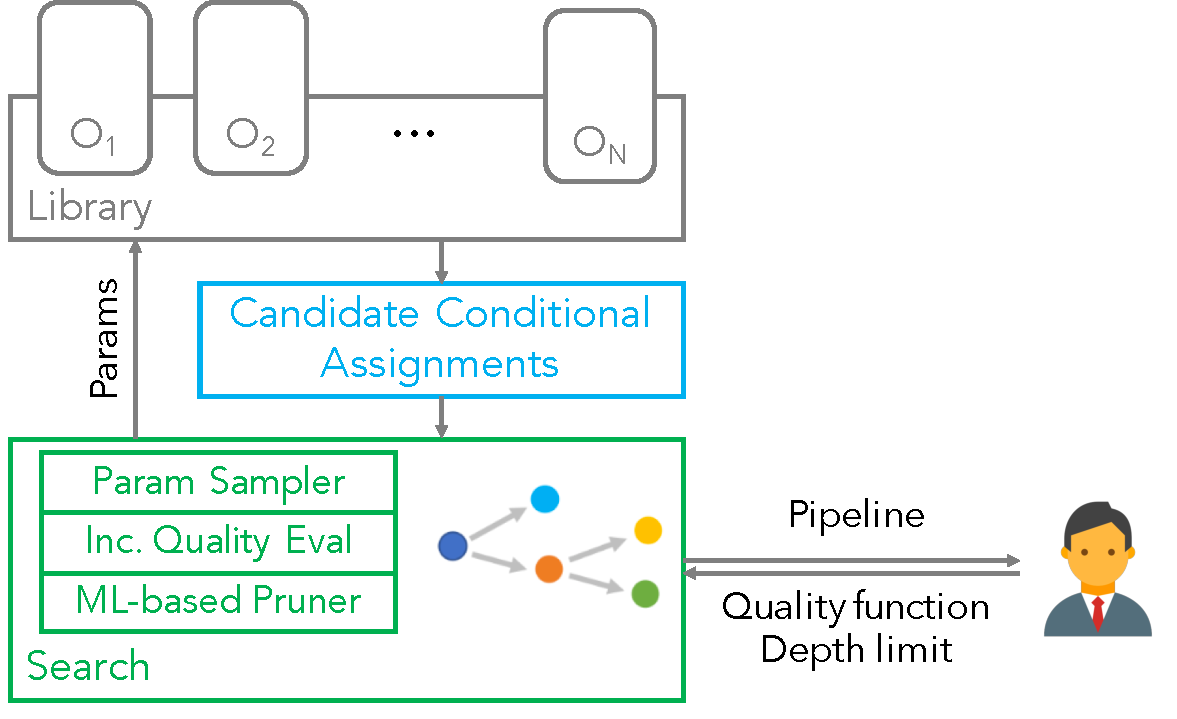
\includegraphics[width=0.7\columnwidth]{figures/arch}
 \caption{\small \sys decouples sampling from the parameter space from search. This allows the user to iterate quickly by observing early best-effort results. \label{fig:arch}}
\end{figure}


\section{Architecture and Overview}
Our goal is to develop a system to automatically generate and tune data cleaning pipelines based on user-specified quality characteristics.  Thus, the user can primarily focus on composing and expressing data quality issues.  We would like the search procedure to be \textbf{progressive}, in the sense that it quickly generates acceptable cleaning plans, and refines those plans over time.  Thus, the user can immediately assess her hypothesis, or test multiple hypotheses in parallel.

\subsection{Interfacing Data Cleaning Frameworks}
The first component of the system is the API interface between existing data cleaning libraries and \sys. We encapsulate the logic of such libraries into a unit we call a \emph{data cleaning framework}, a parametrized function that transforms a dataset. We assume these transformations preserve schema and do not delete/add records.
There are two classes that are important to note, \textsf{Parameter} and \textsf{Repair}.  \textsf{Parameter} is a class that represents the input parameters to a particular framework. \textsf{Repair} is a class that represents the transformations that the framework makes to a given dataset for a particular parameter setting.
\textbf{Section 4 will describe how repairs are represented and composed in more detail.}

Accordingly, each framework is then interfaced to \sys with the following API calls:

\vspace{0.5em}

\noindent Iterates through all possible parameter settings.
\begin{lstlisting}
getParameterSpace(): Iterator<Parameter>
\end{lstlisting}

\noindent Choose a particular parameter setting for the framework.
\begin{lstlisting}
setParameter(Parameter val)
\end{lstlisting}

\noindent Iterate through all repairs that framework would like to apply to the dataset.
\begin{lstlisting}
collectRepairs(): Iterator<Repair>
\end{lstlisting}

\subsection{Quantifying Data Quality}
In machine learning, the objective function for hyper-parameter tuning is often given as the cross validation error of a model. In data cleaning applications, we may not always have objective ground truth. 
A quality function measures a specific notion of cleanliness for a relation, and is used as the objective function for the tuning.  
This is a \emph{proxy} for accuracy defined by the user.
These quality functions are represented in terms of SQL aggregation queries. The user provides a list of SQL aggregates (including UDAF's) and a set of weights to combine these aggregates. 
\textbf{Section 5 describes examples of quality functions and optimizations that we can apply if we have SQL descriptions.}

\subsection{Asynchronous Architecture}
We propose a generate-then-search framework, that decouples the execution of the frameworks and pipeline quality evaluation (Figure~\ref{fig:arch}).  Each framework runs in a separate thread (or process) and continuously reruns with new parameters provided by the {\it Parameter Sampler}.   Its outputs are added to the {\it Repair Pool}.  The Searcher removes repairs from this pool to expand the set of candidate cleaning pipelines, and periodically sends the best pipelines so far to the user.   If the pool exceeds a maximum size, it applies back pressure to pause the cleaning operators until the Searcher has removed a sufficient number of conditional assignments the pool.  In practice, the cost to generate candidate assignments is far higher than the search procedure, and back pressure was not needed in our experiments.   The {\it Quality Evaluator} computes the quality of a candidate pipeline.
To make this framework practical, there are several search optimizations and heuristics that we use.
\textbf{Section 6 describes the search algorithm in detail.}


\subsection{Discussion} 
The key benefit of this asynchronous approach is that the search process does not block on a straggler cleaning framework.  It is common that parameters affect their runtime.  For example, inference thresholds and partitioning parameters can have ``cliffs'', where a small change in parameters can drastically slow down the performance of the method. Including such parameter settings in the search process naively would block the entire system.  In contrast, \sys will simply sample from faster operators until the slow inference task completes.    In fact, this design explicitly highlights the connection between the explored search space and resource scheduling.  For instance,  allocating more CPU resources to more promising operators can affect how the search space is explored.

One drawback of the asynchronous approach is that the Parameter Sampler is oblivious of the search process, so the cleaning operators may generate repairs that are not useful.   The {\it Parameter Sampler} does not attempt to preferentially sample from ``more promising'' parameter spaces, and simply uses uniform sampling.  Similarly, the Library does not perform resource scheduling, and simply allocates one thread per cleaning operator, and each process executes parameter assignments serially. 
We will show that using machine learning to identify promising search paths can alleviate this concern.


% Our main architectural insight is a generate-then-search framework.  Possible parameter values are fed into a library of data cleaning methods, and these parameter assignments asynchronously generate candidate repairs to the dataset (called conditional assignments).  In parallel, a search thread builds a data cleaning plan using compositions of those transformations in the set.  Existing search algorithms implicitly pipeline these two steps; whereas, we decouple these two steps where candidate repairs can be generated in a separate thread and the search algorithm can proceed independently.  This contrasts from the baseline architecture, hereafter called \emph{synchronous tuning}, where a hyperparameter tuning algorithm will then select and assign parameter values to a sequence of operators and evaluate the quality at the end.  There are a few benefits for the asynchronous architecture of \sys.


% \vspace{0.5em} \noindent \textbf{Benefit 2. Progressive Results: } Next, the decoupling also allows for improved progressive behavior with early results. The search thread continuously polls the candidate conditional assignment set for new expansions. The naturally faster  data cleaning methods (e.g., approximate) will generate candidate repairs faster. Slower methods will eventually add these candidate repairs. This allows users to identify faults or glitches in their quality specifications or parameter spaces more quickly than if all methods were synchronously tuned in a pipeline.
